% CREATED BY DAVID FRISK, 2015
\chapter{Methodology}
\label{methodology}
\lettrine[findent=2pt]{\fbox{\textbf{T}}}{ }his chapter is divided in two phases. Each phase has a data collection, data analysis and the implementation. 

%%%%%%
\section{Phase I}

\subsection{Data collection I}
Since Elektra has a lot of data in it, we had to decide on what area to visualize and at which level of abstract. The next sub-section will cover how we ended up deciding on a scope to visualize.

\subsubsection{Identifying a scope to visualize}
As it has been briefly explained in section 2.3, we did the first meeting with Håkan Dahlen at Volvo and he played a big role in identifying the scope of the system to be visualized. We had a long discussion for approximately 2 hours and it was then we figured that we needed to visualize the logical view in Elektra. This view includes the LCs, ports and data elements. \\

If we describe a bit about what is the relationship between ECU and LC is that : first of all, an ECU can have one to many software compositions (SWCs). The SWC is a group of LCs. The LC can have zero to many ports and each port has one data element, it is the data element that connect one LC to another through ports. For example : LC 1 with port 1 can be linked to LC 2 with port 2 only if the port 1 and port 2 has the same data element. Håkan also proposed to visualize the physical view in Elektra which will includes the ECUs.\\

In the discussion with Håkan, we decided to visualize a sub-system. An example of a simple sub-system can be observed from the figure~\ref{fig:hakan-diagram-board} on the top left, there is a small box named SUBSYSTEM and inside of it, there are two ECUs, one ECU has two LCs and another ECU has one LC. The LCs are connected together via ports. The LCs inside the sub-system are also connected to other LCs outside the sub-system but our scope is only for LCs inside a single sub-system. So for this report, we will visualize a sub-system named Visibility Control SPA, this sub-system has 18 LCs and 179 ports at the moment.\\


\begin{figure}[H]
\centering
\captionsetup{justification=centering}
\vspace{0cm}% Adjust vertical spacing here
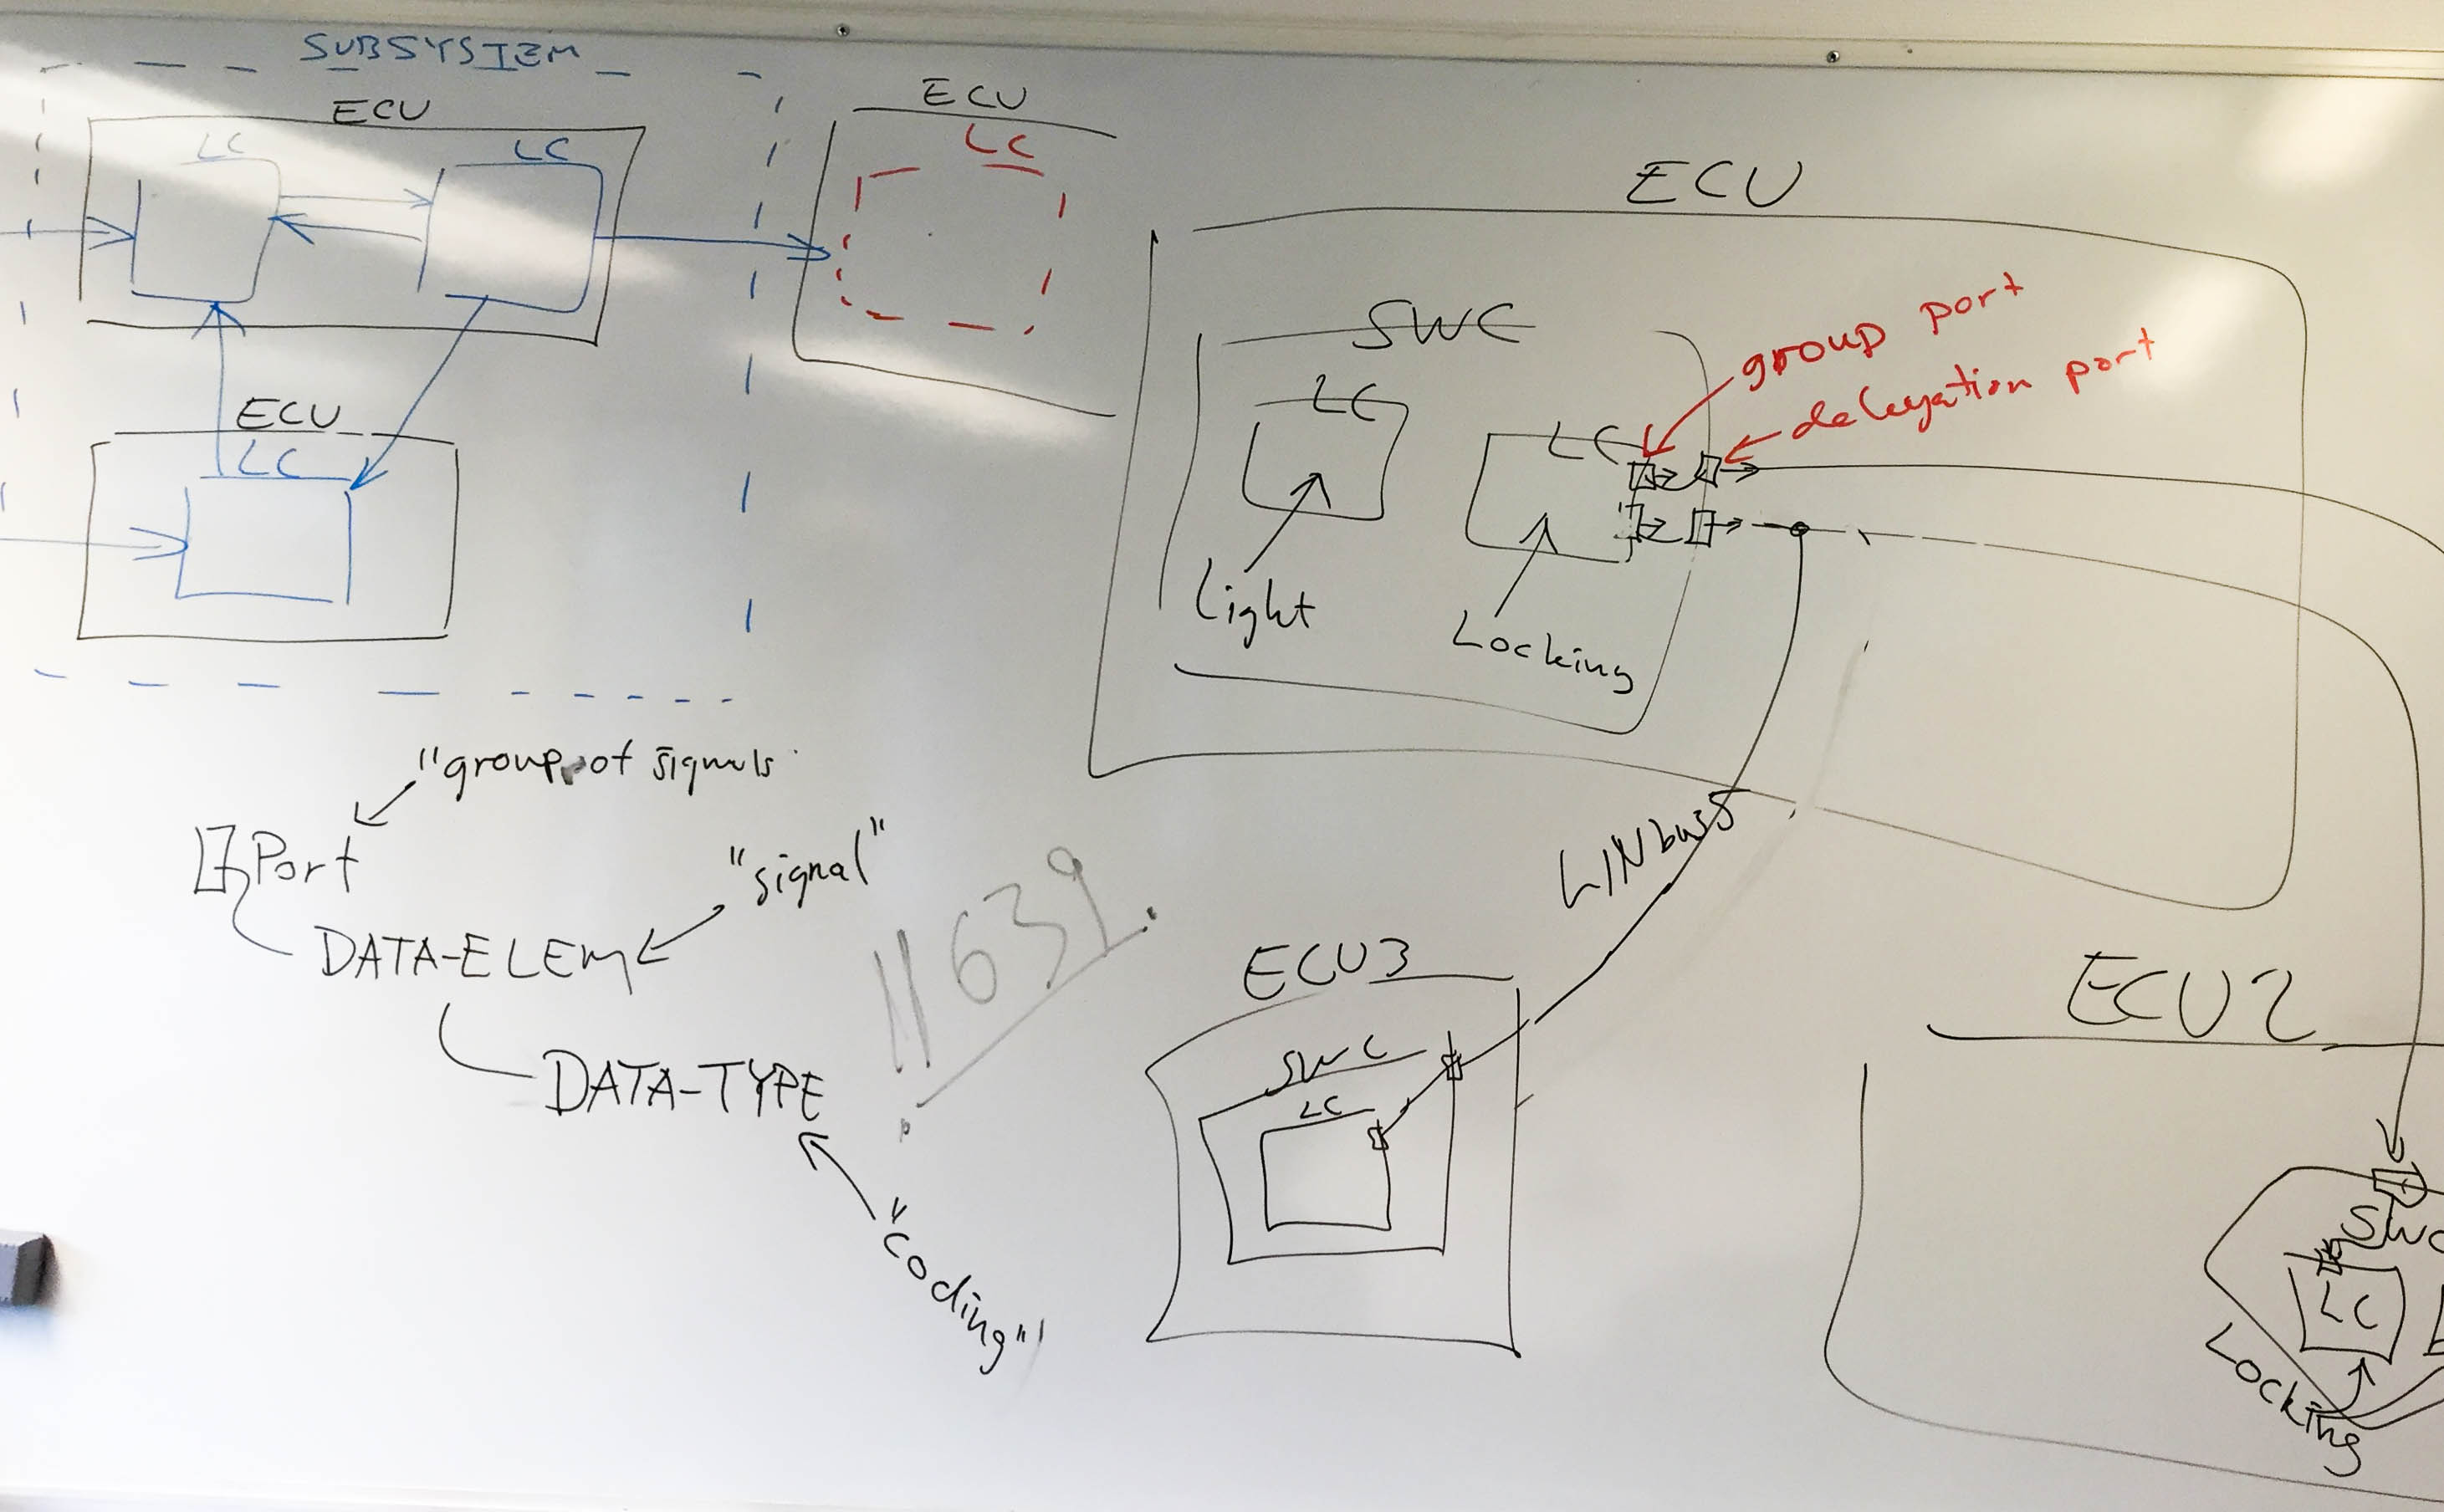
\includegraphics[width=0.85\linewidth]{figure/misc/Hakan.jpg}
\caption{Example of a visualization from a stakeholder}
\label{fig:hakan-diagram-board}
\end{figure}

\subsubsection{Extracting data from Elektra}
The best way that was suggested in retrieving data from Elektra was to use an application program interface(API). At Volvo, we were given a documentation that has a list of APIs and the description of how to use the APIs in order to get the data of your need from Elektra. In order to access the data, one has to be within the Volvo network. Since we did most of our studies outside the company area then we were forced to use the censored data file. The use of API is more dynamic than visualizing a single static file of data. However, this does not make the step to retrieve data from Elektra less meaningful, it is still the same data but later on, a static file will need to be replaced with a specific API url to get the data from Elektra.\\

The data found in the static file retrieved from Elektra is in JavaScript Object Notation(JSON) format. A simple example of JSON object is shown in the  Listing~\ref{code:report_JSON_Object} below :

\begin{lstlisting}[caption=An example of JSON object, label=code:report_JSON_Object]
{
    "id": 1,
    "name": "Master Thesis report",
    "year": 2016,
    "place" : "Sweden",
    "examiner" : "Eric",
    "Supervisors": ["Truong", "Ulf", "Michel","Patrizio"]
}
\end{lstlisting}

%%%%%%
\subsection{Data analysis I}

\subsubsection{Analyzing the raw JSON data}

On this sub-section, we had to understand the meaning of the objects found in the JSON static file and also how most of the objects were connected. The static file had approximately 45 thousands line of code. The beginning of the static file that was retrieved from Elektra is shown in the Listing~\ref{code:origin_static_file} below:

\begin{lstlisting}[caption=A small part of how the original file appear, label=code:origin_static_file]
{
   "elementName": "Visibility Control SPA", 
    "name": "Visibility Control SPA", 
    "state": "In work", 
    "classType": "GSUBSYSTEM", 
    "variant": "MAIN", 
    "domain": "VCC_EEDM", 
    "creationUser": "Anonymous", 
    "className": "SUBSYSTEM", 
    "contentRelations": [
        {
            "destination": {
                "elementName": "LTC 1", 
                "name": "Name for LTC 1", 
                "classType": "GLTC", 
                "variant": "MAIN", 
                "domain": "VCC_EEDM", 
                "creationUser": "Anonymous", 
                "className": "LTC", 
                "state": "Frozen", 
                "modificationUser": "Anonymous", 
                "modificationDate": "2013-06-25T05:13:36+0000", 
                "attributes": {
                    "MaximumLatency": "250", 
                    "Access control": "Access allowed", 
                    "NominalLatency": "-1", 
                    "RefinedConstraints": [], 
                    .....
                }, 
                "creationDate": "2013-05-02T11:48:25+0000", 
                "id": "1937212", 
                "elementId": "1169278", 
                "revision": 0
            }, 
            "contentAttributes": {}
        }, 
        .....   
}
\end{lstlisting}

From the Listing~\ref{code:origin_static_file} shown above, the variable "elementName" that appears on the first row of the JSON file specifies the name of the sub-system that is visualized which has the value "Visibility Control System". You can also notice the variable "className" that appears on the 8th row of the JSON file which has the value "SUBSYSTEM". \\

In order to explain the relationships between JSON objects found in a static flie, we created a meta-model which can help to understand the data found in the file, see figure~\ref{fig:old_metamodel} below.

\begin{figure}[H]
\centering
\captionsetup{justification=centering}
\vspace{0cm}% Adjust vertical spacing here
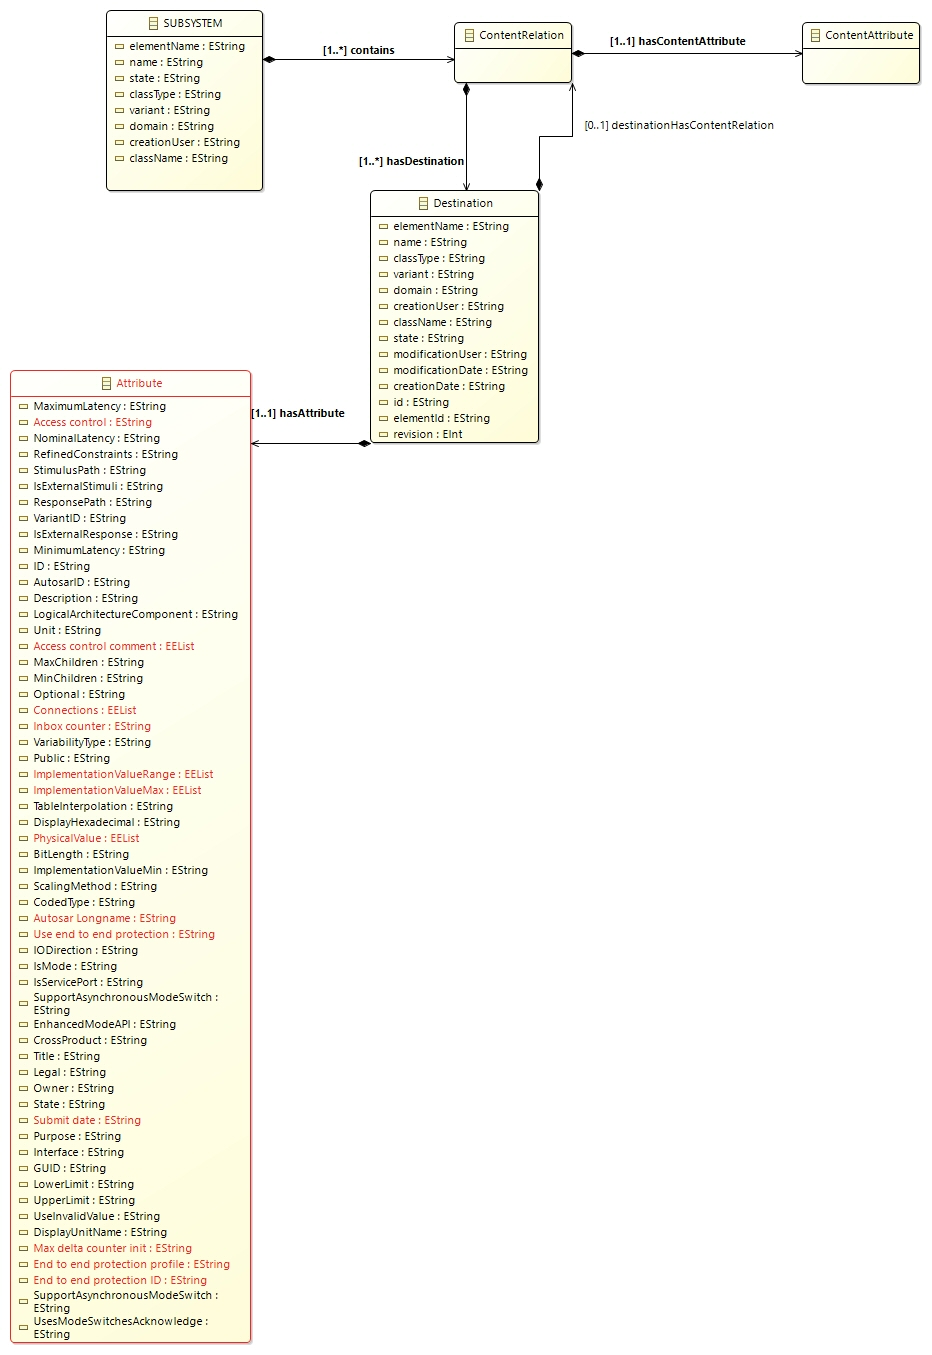
\includegraphics[width=0.85\linewidth]{figure/new_model/Old_Metamodel.jpg}
\caption{Old metamodel}
\label{fig:old_metamodel}
\end{figure}

The meta-model shown in the figure~\ref{fig:old_metamodel} has sum up most of the variables found in the JSON file. The classes that we needed the most are the "contentRelations", "destination" and "attributes". You can notice that the class "contentRelations" has an association of one to many with the class "destination" and also the class "destination" has an association of zero to one with the class "contentRelations". The class "destination" has an association of one to one with the class "attribute". \\

The objects of the class "destination" could be LC, port, data-element, data-type, REQSET, etc. In order to elaborate this, we will give an example of how it appears in a JSON file (see the lists that follows) and the Listing~\ref{code:lc_port_dataElem} after it : \\

\begin{enumerate}
\item a LC which is an object of a class \texttt{destination} has an object of a class "contentRelations",call it CR1,
\item an object CR1 can have an array of objects of a class "destinations", a port being one of the object of a class  "destination",
\item a port has an object of a class "contentRelations", call it CR2,
\item an object CR2 can have an array of objects of a class "destinations", a data-element being one of the object of a class "destination",
\item a data-element has an object of a class "contentRelations", call it CR3,
\item an object CR3 can have an array of objects of a class "destinations", a data-type being one of the object of a class "destination", etc \\
\end{enumerate} 

\begin{lstlisting}[caption={A sample part of a JSON file showing the relationship between a LC, a port and a data-element},label=code:lc_port_dataElem]
{
  "destination": {
      "elementName": "LC 1", 
      "name": "Name for LC 1", 
       ....., 
      "contentRelations": [
            {
            "destination": {
                "elementName": "PORT 1", 
                "name": "Name for PORT 1", 
                  ....., 
                 "contentRelations": [
                      {
                      "destination": {
                           "elementName": "DATA-ELEM 1", 
                           "name": "Name for DATA-ELEM 1", 
                            .... 
                           "contentRelations": [
                                 {
                                  "destination": {
                                  "elementName": "DATA-TYPE 1", 
                                  "name": "Name for DATA-TYPE 1",    .....,   
                "attributes": {
                    "IODirection": "REQUIRE",
                    ...
}\\
\end{lstlisting}

If you take a look again at the Listing~\ref{code:lc_port_dataElem}, you can notice a variable with the name "attributes" near the end. This variable has another variable inside of it with the name "IODirection". The variable "IODirection" determines whether a port provides to another port or a port requires another port. The principle in this context of require and provide is that it explains about a dependencies between ports and when it comes to visualize the connection between LCs, we take a look at this variable to determine on how to map the ports in a component diagram.\\

how it looks like, previous meta model, why it doesn't work out \todo{[to be filled in]}


%%%%%%
\subsection{Implementation I}
The data retrieved from Elektra had so many information that were somehow not needed in the visualization. The first step we did was to find a way to omit the data that was not needed and keep the one that we only needed to visualize and that was the names of the LCs, names of the ports, the value of port that determines whether a port requires another port or a port provides to another port and also we need to keep the data element for each port.

\subsubsection{Optimizing the raw JSON data}
As you can see in the previous listing, the json data had lots of information that was necessary to be filtered. What we did was to write a java code that is able to read the original json data and get only the data that we will have used to do the visualization. Some of the JSON object that we had remained with are specifically the names of LCs, the ports for each LCs, the name of the ports, the IODirection of the port which determines the connection between the ports and and the name of the data element of the port.\\

A sample code can be seen in the listing below where we first read a contentRelations JSON object to get its destinations, so first of all we get the LC, then an LC has a contentRelation JSON object and inside the object, it has a list of destinations. Now, we have a port JSON object, the port has element name and has an attribute JSON object which inside of it, the IODirection value can be retrieved. Finally we needed the name of the data element. The port JSON object is a destination that has a contentRelation JSON object, again, this object has destinations, on of the destination being a data element. The loop keeps on repeating until it has finished with all the LCs. Once the loop has finished, it saves the resulted JSON contents to a new file and this file will now be a model instance. \\

To explain how the algorithm works, we will write down the steps that we follow :
\begin{enumerate}
\item Read from a original JSON file
\item Get the name of the susbsytem
\item Introduce loop 1 that gets all the LCs of the subsystem.
\item Introduce loop 2 inside loop 1 that gets all the ports of a single LC
\item Get the name of the port
\item Get the name of the data-element
\item Get the value value of \texttt{IODirection} of the port
\item End of the loop 2 
\item End of the loop 1
\item Write an optimized content to a new file
\end{enumerate}

The result of the above explanation appears in the listing below :

\begin{lstlisting}[caption=A sample part of the optimized JSON content,label=code:optimized_JSON]
{
  "elementName": "Visibility Control SPA",
  "hasLC": [
    {
      "elementName": "LC 1",
      "hasPort": [
        {
          "elementName": "PORT 1",
          "IOdirection": "REQUIRE",
          "dataElement": "DATA-ELEM 1"
        }
      ]
    },
    {
      "elementName": "LC 2",
      "hasPort": []
    },
    {
      "elementName": "LC 3",
      "hasPort": [
        {
          "elementName": "PORT 2",
          "IOdirection": "REQUIRE",
          "dataElement": "DATA-ELEM 2"
        },
        {
          "elementName": "PORT 3",
          "IOdirection": "REQUIRE",
          "dataElement": "DATA-ELEM 3"
        }
        ....
}
\end{lstlisting}


\subsubsection{Creating a new meta-model and model instance}
Once the raw JSON data is optimized (Listing~\ref{code:optimized_JSON}), we created a meta-model and a model instance using the open-source tool JSON discoverer. Before getting to the point where we obtained the meta-model and the model instance, we want to explain how the discovering of JSON schema process work. Based on the paper written by the tool creators Javier Luis Cánovas Izquierdo and Jordi Cabot~\cite{Canovas}, the discovering process is a model-based process which is composed of three phases:  pre-discovery phase, single-service discovery phase, and multi-service discovery
phase. The first phase aims to extract the low-level a JSON model out of a JSON document. The second phase is to obtain the schema information of a JSON document. The last phase aims at obtaining common schema of more than one JSON documents. Since the data of the sub-system Visiblity Control System that we extracted from Elektra was in one single JSON document, multi-service discovery phase was not used. \\

With the optimized version of the raw JSON file, JSON discover provided us a very-simple-but-efficient meta-model. From Figure~\ref{fig:new_metamodel}, the meta-model comprises three classes \texttt{SubSystem}, \texttt{HasLC}, and \texttt{HasPort}. Each class has one or more attributes. \texttt{SubSystem} has an attribute \texttt{elementName} keeping the name of sub-system. The class \texttt{HasLC} has one attribute \texttt{elementName} keeping the name of LC. The class \texttt{HasPort} has three attributes namely \texttt{elementName} containing the name of port, \texttt{IODirection} specifying the type of port (\texttt{PROVIDE} or \texttt{REQUIRE}), and \texttt{dataElement} keeping the name of port. All attributes are \texttt{String} type of value.

\begin{figure}[H]
\centering
\captionsetup{justification=centering}
\vspace{0cm}% Adjust vertical spacing here
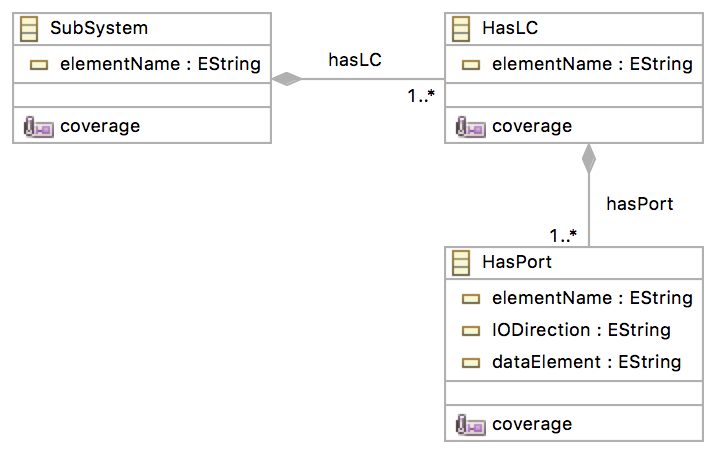
\includegraphics[width=0.65\linewidth]{figure/new_model/new_metamodel.png}
\caption{The meta-model of the optimized JSON document discovered by JSON discoverer tool}
\label{fig:new_metamodel}
\end{figure}

The meta-model also has two class relationships: \texttt{hasLC} and \texttt{hasPort}. The first relationship is a composition meaning that the class \texttt{HasLC} will be destroyed if the class \texttt{SubSystem} is destroyed. The same type of relationship is also applied to the relationship between the class \texttt{HasLC} and \texttt{HasPort}. Both relationships have multiplicity \texttt{1..*} according to the optimized JSON document. Note that the annotations \texttt{coverage} included in all classes are resulted from the the JSON grammar rules the authors of JSON discoverer created to guide the generation of the JSON meta-model~\cite{Canovas}. \\

As it has been mentioned that JSON discoverer also provides the discovery of data model (model instance). Using the same optimized JSON document, we obtained a model instance in XML\footnote{Extensible Markup Language} Metadata Interchange (XMI) file. A part of the file can be seen in Listing~\ref{code:model_instance_xmi}.

\begin{lstlisting}[caption=Data model or model instance discovered by JSON discoverer,label=code:model_instance_xmi]
<?xml version="1.0" encoding="UTF-8"?>
<discoD:SubSystem
    xmi:version="2.0"
    xmlns:xmi="http://www.omg.org/XMI"
    xmlns:xsi="http://www.w3.org/2001/XMLSchema-instance"
    xmlns:discoD="http://jsonDiscoverer/discovered/SubSystem"
    xsi:schemaLocation="http://jsonDiscoverer/discovered/SubSystem metamodel.ecore" elementName="Visibility Control SPA">
  <hasLC elementName="LC 1">
    <hasPort elementName="PORT 1" IODirection="REQUIRE" dataElement="DATA-ELEM 1"/>
  </hasLC>
  ...
</discoD:SubSystem>
\end{lstlisting}

Using the editor from the EcoreTools Eclipse plug-in, the model instance is visualized as seen in Figure~\ref{fig:new_model_instance}.

\begin{figure}[H]
\centering
\captionsetup{justification=centering}
\vspace{0cm}% Adjust vertical spacing here
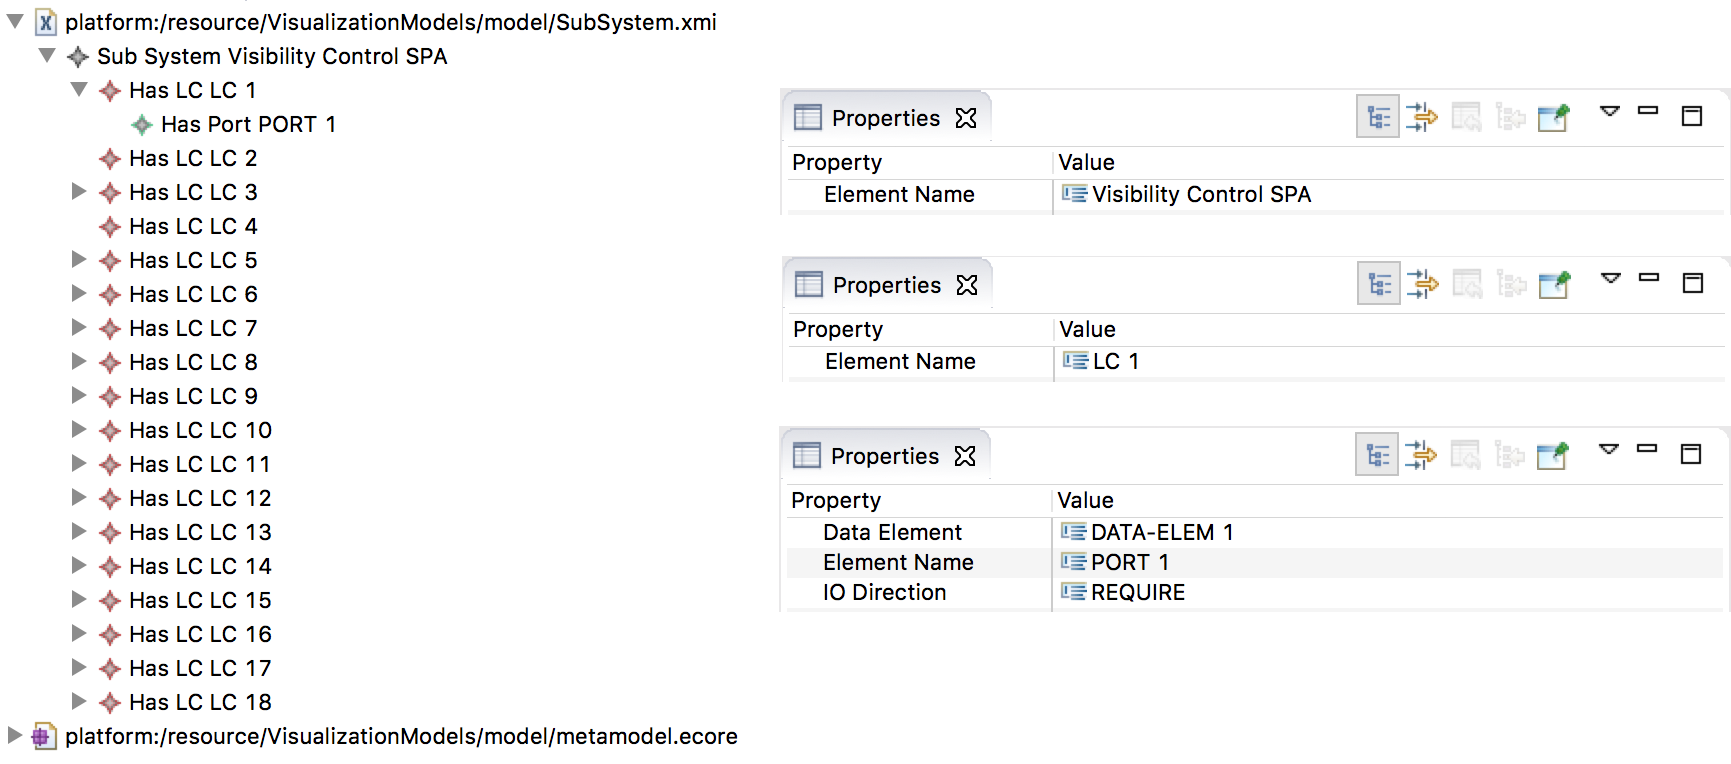
\includegraphics[width=0.6\linewidth]{figure/new_model/new_model_instance.png}
\caption{}
\label{fig:new_model_instance}
\end{figure}

\subsubsection{Creating a visualization using Acceleo and PlantUML}
\todo{[to be filled in]}


%------------------------------------------------------------------%
%%%%%%
\section{Phase II}

\subsection{Data collection II}

\subsubsection{Preparation for the interview}
The article \cite{Basili} has explained couple of steps to follow when collecting data. We have applied the first two steps mentioned in article \cite{Basili}, the steps are establishing the goals for data collection and developing a list of questions of interests. The goals we have set for this interview are getting to knowing important artifacts on the visualization output from the each stakeholder, getting to know the artifacts that most stakeholder needs in their line of work, finding the metrics that we can use to determine the important artifacts and also understanding the needs of the stakeholders. 

\subsubsection{Selecting a group of stakeholders}
Since the visualization is based on a single subsystem namely Visibility Control SPA, we would prefer to interview the stakeholders that uses this subsystem often. These are the primary stakeholders since they are directly interacting with the ELektra.

\subsubsection{Interviewing the selected stakeholders}
\todo{[to be filled in]}

%%%%%%
\subsection{Data analysis II}

\subsubsection{Identifying the needs of the stakeholders}
\todo{[to be filled in]}

\subsubsection{Discovering metrics}
\todo{[to be filled in]}

%%%%%%
\subsection{Implementation II}

\subsubsection{Applying the metrics to the visualization}
\todo{[to be filled in]}
